\documentclass[a4paper]{article}
%%%%%Paquetes%%%%%
\usepackage[T1]{fontenc}
\usepackage[utf8]{inputenc}
\usepackage[english]{babel}
\usepackage{amsmath,amssymb,eucal,mathrsfs}
\usepackage[svgnames,x11names]{xcolor}
\usepackage{colortbl}
\usepackage{Estilos/MiEstilo}
%\usepackage{Estilos/Informe}
\usepackage{amsmath}
\usepackage{times}
\usepackage{color}
\usepackage{listings}
\usepackage{graphicx}
\usepackage{caption}
\usepackage{float}
\usepackage[]{algorithm2e}
	\setcounter{tocdepth}{2} %Mostrar solo 3 niveles en el índice
		\makeindex	%índice de palabras
		\title{Computational Complexity\\ Assignment 2 }
		\author{Luis José Quintana Bolaño}
		\date{\today}

\begin{document}
	\maketitle
	\begin{abstract}
	    This document examines the design and implementation of a naïve algorithm for the Stainer Tree problem (ST). It provides the worst-case time analysis, the design of a parametric graph for experimentation and observations of the experiments conducted on this graph for 0 to 20 optional graphs.
  	\end{abstract}
  	
	\section{Introduction}
	    In this assignment we are required to propose a solution for the Steiner Tree problem.
	    
	    The Steiner tree problem is very similar to the minimum spanner tree, in the sense that both are required to find the network (graph) of shortest length (i.e. the sum of the length of all edges) that interconects all given vertex, with the difference being that, in the Steiner tree problem, optional vertices and edges may be added to the graph in order to reduce the length of the spanning tree. It's been proven that the solution is always a tree, and several trees may solve the same given set of initial vertices.
		    \begin{figure}[!h]
  			\centering
  			\includegraphics[width=0.55\textwidth,clip]{Graph.png}
  			\caption{Example of the reduction of the spanning tree with three initial vertices by adding an optional one.}
  			\end{figure}
  		%\subsection{Analysis}
  		%    Assuming that each transition takes precisely one time unit, we conclude, upon close examination of the automaton, that the time function is $ T(n)=\frac1 2 n^2+\frac3 2 n+3+n\bmod2 $, and thus: $T(n)\in O(n^2)$
    %\newpage
    
    
    \section{Implementation}
    As required in the assignment, the Steiner tree problem solver has been implemented in C++.
    
    Since the problem is a variation on the minimum spanning tree problem, Prim's algorithm has been used as a base, implemented according to the pseudocode provided witht the documentation for the assignment.
    
    In order to find the Steiner tree, the computation of Prim with every single possible combination of optional vertices is necessary, to find the shortest one. For the generation of the k-combinations, a recursive solution has been proposed, in wich the recursive function includes one of the optional vertices in the graph (received as a parameter), then computes Prim and calls itself with the current graph and the next vertex to be included for all optional vertex remaining, returning the minimum value between it's own computed Prim and those returned by the recursive calls. This process continues until all possible combinations have been tested, thus obtaining the minimum spanning tree amongst all posible graphs (i.e. the Steiner tree).\newpage

\begin{algorithm}[H]
 \KwData{Graph $G$, Vertex $V$}
 \KwResult{minimum ST found by Prim's algorithm }
 Include vertex $V$ in graph $G$\;
 Set $Prim(G)$ as current best result \;
 \For{every optional Vertex after $V$, $O_i$}{
  \If{current best $>$ recursive call($G$, $O_i$)}{
   Set recursive call's result as current best\;
   }
 }
 \Return current best\;
 \caption{Recursive steiner function}
\end{algorithm}

    \section{Analysis}
        \subsection{Worst-case time}
            As our algorithm tries Prim on every possible combination of optional vertices, for $n$ vertices it must do $2^{n}$ iterations of Prim, which itself belongs to $O(n^2)$
            Tu función, sea recursiva o no, tiene que generar 2^n combinaciones
Y dentro de esa función también llamas a prim
Que es orden n^2
Pues ya sabes que ese es el orden
Puede tener otras funciones que se llamen, pero la mayor es esa
Así más o menos lo he hecho
no me queda muy claro
que es entonces, 2^n, independientemente de que sea recursiva o no?
Siempre que las demás funciones que se llaman en el bucle de 2^n sean menor que esa sí
Porque por la regla del máximo, te quedas con la mayor
Ahora te lo explico mejor
si tienes una función que llama a varias
y son dos, una de valor n y otra n^2
sería así
2^n(n+n²)
que es lo mismo que 2^n*n + 2^n*n²
haciendo la regla del máximo
se ve que el mayor es 2^n*n²
ése sería el coste
        \subsection{Experiments}
        \subsection{Observations}
        
        \subsection{Observed Time Complexity}
            \begin{figure}[!h]
  			\centering
  			%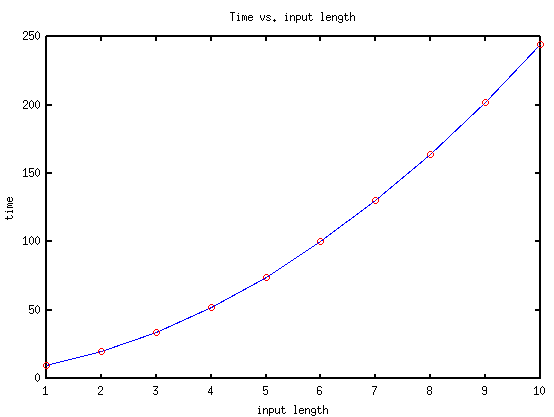
\includegraphics[width=0.55\textwidth,clip]{timecomparatorturing.png}
  			\caption{Plot of the time vs. input length for the turing machine implementation of the binary comparator.}
  			\end{figure}
  		\subsection{Analysis}
  		    Assuming that each transition takes precisely one time unit, we conclude, upon close examination of the automaton, that the time function is $ T(n)=2 n^2+4 n+4 $, and thus: $T(n)\in O(n^2)$
    \section{The RAM model}
        \subsection{Binary Palindrome Decider}
            \begin{figure}[!h]
  			\centering
  			\begin{tabular}{r|c|c|c|c|c|c|c|c|c|c|} \hline
  				input length  & 1 & 2 & 3 & 4 & 5 & 6 & 7 & 8 & 9 & 10 \\ \hline
  				time          & 35 & 39 & 56 & 60 & 77 & 81 & 98 & 102 & 119 & 123 \\ \hline
  		    \end{tabular} \\
  		    \end{figure}
  		    In this case, we can observe a time function $ T(n)\in O(n)$
        \subsection{Binary Comparator}
            \begin{figure}[!h]
  			\centering
  			\begin{tabular}{r|c|c|c|c|c|c|c|c|c|c|} \hline
  				input length  & 1 & 2 & 3 & 4 & 5 & 6 & 7 & 8 & 9 & 10 \\ \hline
  				time          & 34 & 49 & 64 & 79 & 94 & 109 & 124 & 139 & 154 & 169 \\ \hline
  		    \end{tabular} \\
  		    \end{figure}
  		    In this case, we can observe a time function $ T(n)=15n+19 $, and thus: $T(n)\in O(n)$
  		\subsection{Conclusion}
  		    In both machines the computations remain in polynomial time.
		
\end{document}
